%% LaTeX2e class for seminar theses
%% sections/content.tex
%% 
%% Karlsruhe Institute of Technology
%% Institute for Program Structures and Data Organization
%% Chair for Software Design and Quality (SDQ)
%%
%% Dr.-Ing. Erik Burger
%% burger@kit.edu

\section{Brauchen wir (russisches) Erdgas?}
\label{ch:Introduction}

%% -------------------
%% | Example content |
%% -------------------

Deutschland bezog 2020 mit 500 TWh Erdgas 55\% des Gesamtbedarfs aus Russland \cite{clausen2022}. Russland exportiert umgekehrt mit etwa 25\% das meiste Erdgas nach Deutschland \cite{iwd}. 
Diese Zahlen verdeutlicht, dass Deutschland stark abhängig von russichem Gas ist. Russland mag in der Lage sein andere Abnehmerländer für das Gas zu finden. Ein schnelles vollständiges Embargo würde die russischen Einnahmen aus Erdgas dennoch stark reduzieren. Solange Deutschland diese Handelsbeziehung fortführt finanziert es indirekt den russischen Angriffskrieg auf die Ukraine mit.

Die Lage der Energieversorgung im Frühjahr 2022 wurde dadurch verschärft, dass Stand 05.03.~die deutschen Erdgasspeicher nur zu 27\% gefüllt waren, wohingegen sie im selben Zeitraum normalerweise bis zu 50-80\% gefüllt sind \cite{leo}. Am 30.03.~rief das Bundesministerium für Wirtschaft und Klimaschutz (BMWK) die Frühwarnstufe des Notfallplans Gas aus \cite{bmwk}. Das bedeutet, dass zwar die Versorgungssicherheit weiterhin gewährtleistet war, aber Vorsorgemaßnahmen getroffen wurden und jeder Verbraucher angehalten ist seinen Verbrauch so gut wie möglich zu reduzieren.

Russland drohte mit einem Gaslieferstopp wenn Gaszahlungen nicht in Rubel beglichen werden \cite{bmwk}.
Am 15.06.~ schickte Gazprom nur noch 0.7 statt den üblichen 1.7 TWh/d (= 59\%) durch die Nord Stream Gasleitung \cite{gazprom-gasverknappung}. Der dafür genannte Grund sind durch Lieferschwierigkeiten verzögerte Reparaturarbeiten, doch diese Begründung wird vielerseits angezweifelt. Aufgrund der hohen Abhängigkeit eignet sich die Einstellung oder Reduktion der Gaslieferungen für Russland als sehr gutes Druckmittel gegenüber dem die Ukraine unterstützenden Deutschland. 
%Gasknappheit ist in den warmen Sommermonaten weniger problematisch als es womöglich im kommenden Winter der Fall sein wird

Deutschland muss alternative Quellen für russisches Erdgas verwenden oder den Erdgasverbrauch reduzieren. In den Folgenden Abschnitten wird ergründet ob und wie dies möglich ist.

\subsection{Direkter Ersatz durch Importe}
% A citation: \cite{becker2008a} For referencing, see \autoref{sec:Introduction:Figures}

\begin{figure}
\centering
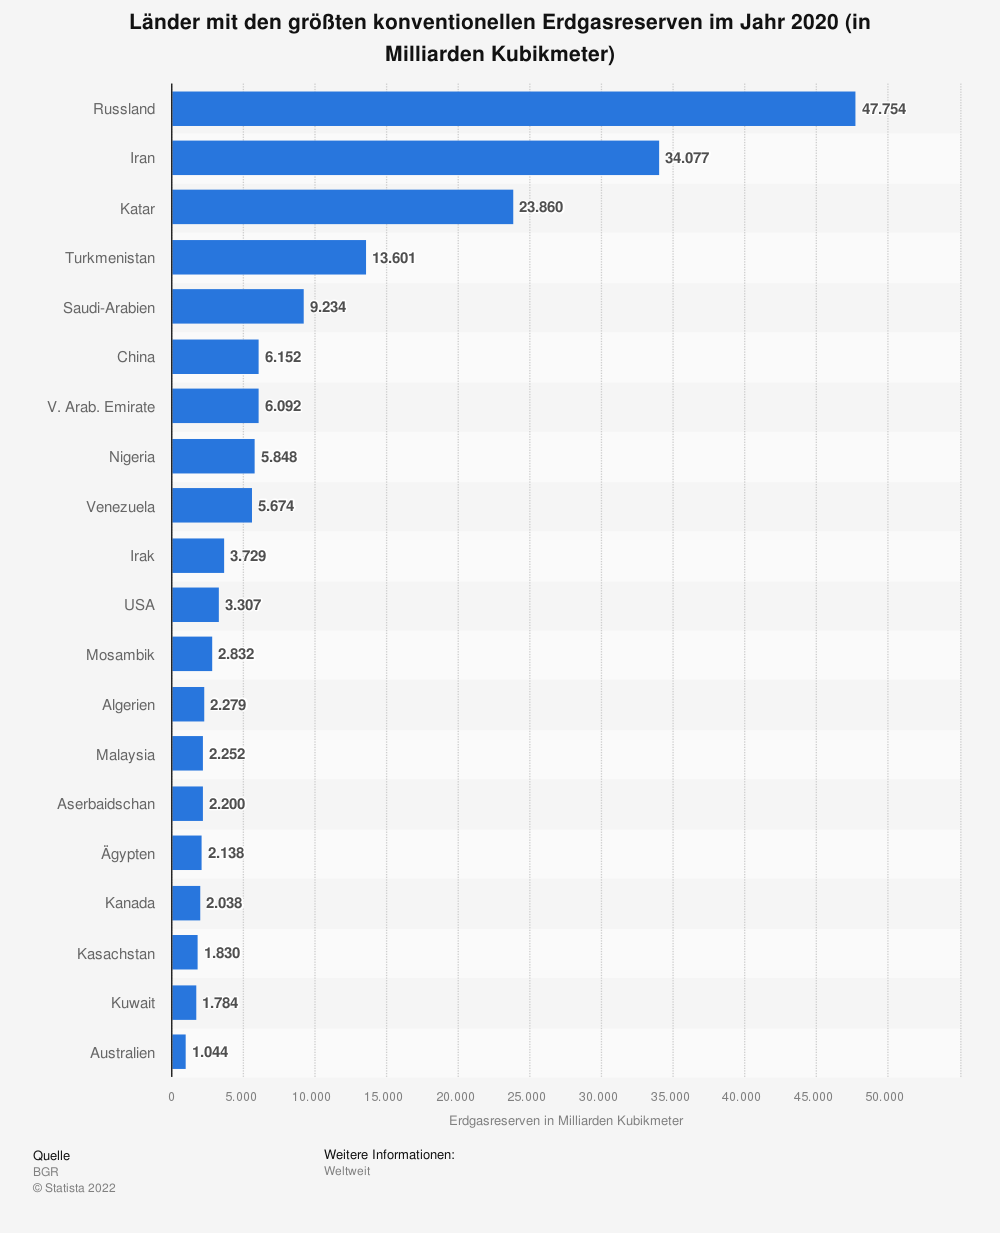
\includegraphics[width=8cm]{../pres/fig/erdgasreserven.png}
\caption{Länder mit den größten konventionellen Erdgasreserven 2020 (in Milliarden Kubikmeter) \cite{statista-erdgasreserven}}
\label{fig:erdgasreserven}
\end{figure}

Russland ist 2020 mit über 500.000 TWh weltweit das Land mit den größten konventionellen Erdgasreserven. \autoref{fig:erdgasreserven} zeigt, dass auch für die Politik der nächsterdgasreichsten Ländern eine Tendenz zur Autokratie beobachtet werden kann. 

Der Theorie des ``Fluches der Rohstoffe'' oder auch ``Paradox of Plenty`` sieht eben genau im Rohstoffreichtum dieser Länder dafür eine mögliche Erklärung \cite{gabler}. Rohstoffreichtum kann ein Chance aber auch eine Herausforderung in der Entwicklung eines Landes sein. Werden die Rohstoffe gut genutzt, können sie für verbreiteten Wohlstand sorgen. Schlecht genutzt sorgen sie für Instability, soziale Konflikte und Umweltschäden. 
Rohstoffe können strategischer Natur wie Energieträger, aber auch industrieller (z.B.~Kupfer) oder gewinnträchtiger (z.B.~Diamanten) Natur sein.

Eine erklärende Theorie ist dass Regierungen wahrscheinlicher zu demokratischen Elementen übergehen, wenn ihr fiskales Budget abhängig von Steuern ist \cite{nrgi}. Existieren wertvolle natürliche Ressourcen im Land und werden diese von nur wenigen Menschen oder Unternehmen kontrolliert, kann ein Großteil des nationalen Budgets aus dieser Richtung kommen. Damit ist eine Regierung weniger abhängig davon die Bürger zu befriedigen und umgekehrt sind Bürger weniger darauf aufmerksam, was mit dem nationalen Budget gemacht wird. 

Konflikte über die Kontrolle der Rohstoffe sorgen für Instabilität im Land. Ölproduzierende Länder leiden doppelt so wahrscheinlich unter Bürgerkriegen und sind häufiger Ziel internationaler Kriege (``petro-aggression'') \cite{nrgi}.

Doch ein Zuwachs an natürliche Rohstoffen können auch negative wirtschaftliche Auswirkungen auf andere Sektoren haben \cite{nrgi}. Dieses Phänomen wird auch ``holländische Krankheit'' bezeichnet, in Anlehnung an den Rückgang des niederländischen produzierenden Sektor nach Entdeckung des Groninger Erdgasfeldes 1959. Ein höheres Maß an Rohstoffen stärkt die nationale Währung und macht damit Importe günstiger und Exporte teurer, was auf lange Sicht die Wettbewerbsfähigkeit des produzierendes Gewerbes schwächt.

Diese Erklärungen deuten darauf hin, dass Erdgasimporte jeglicher Art und Herkunft tendenziell den bitteren Beigeschmack haben, dass man damit hilft elitäre Herrschaftssysteme in diesen Ländern aufrechtzuerhalten.

Die (langfristige) Notwendigkeit von Erdgas wird in späteren Abschnitten evaluiert. Für manche Verbraucher ist der kurzfristige Ersatz durchaus schwierig, weswegen ein Ersatz aus anderen Ländern trotz beschriebener Problematik kurzfristig angestrebt wird. Erdgas kann entweder als gasförmiger Energieträger über Pipelines importiert werden oder über längere Strecken in flüssiger Form auf Behältern in Schiffen transportiert werden. Diese Form wird auch Flüssiggas oder Liquid Natural Gas (LNG) genannt. Pipeline-Importe sind den LNG-Importen im Allgemeinen aus verschiedenen Gründen vorzuziehen. 

Zum Ersten ist die Umwandlung in Flüssiggas, der Transport über weite Wege und die Wiederaufbreitung zu Gas deutlich energieintensiver, damit teurer und mit höheren Emissionen verbunden \cite{lng-faq}. 
Darüber hinaus hat Deutschland und die EU (noch) keine ausreichende Infrastruktur um Flüssiggas am Meer zu empfangen und die Importe ins Landesinnere weiterzutransportieren \cite{iwd}. Deutschland besitzt bisher noch keine LNG-Terminals, die Anbindung anderer EU-Nachbarländer ist jedoch gut. 
Die Umschlagskapazität der Terminals ist nicht ausgereizt: die Importkapazität der LNG-Terminals der 27 EU-Länder liegt bei 1715 TWh wovon nur 798 TWh tatsächlich genutzt werden \cite{leo}. Zusätzlich verfügt die Türkei die über mehrere LNG-Terminals. 


Deutschland mit den Flüssiggas-Beschleunigungsgesetz 11 LNG-Terminals für Deutschland, was einer Importkapazität von 286 TWh entsprechen wird \cite{lng-gesetz}. Teile davon werden als schwimmende Anlagen errichtet. Der Bau stößt bei Umweltverbänden wegen einer möglicher Gefährdung von Schweinswalen auf Kritik.
Schwierig ist der Weitertransport durch Gasleitungen vor allem aufgrund fehlender Pipelines von Spanien nach Mitteleuropa \cite{iwd}.
Langfristig wird die Klimaneutralität angestrebt. Das stellt die Investition in teure Infrastruktur, die neben Erdgasimporten womöglich keinen anderen Zweck erfüllt infrage. Deswegen ist beim Bau auf die Fähigkeit zur Umstellung auf einen Transport von Wasserstoff statt Erdgas (H2-ready Konzept) zu beachten \cite{leo}.

Neben der Frage, ob Deutschland in der Lage ist Importe zu empfangen ist zu klären aus welchen Ländern Erdgas importiert werden kann. Kurzfristig soll die Produktion innerhalb der EU und Importe aus nicht-russischen Gebieten (insbesondere Aserbaidschan und Norwegen) um 106 TWh im Vergleich zu 2021 erhöht werden können \cite{iea2022}. Diese Erhöhung geht auf eine höhere Nutzung der Kapazitäten und Vorkommen, übersprungene Wartungen im Sommer und eine Erhöhung der Produktionsgrenzen zurück, was die längerfristige Anwendbarkeit dieser Strategie infragestellt. Des Weiteren ist die EU-weite Erhöhung um 106 TWh bei Weitem nicht in der Lage die existierende Nachfrage zu decken.

Zu den möglichen Herkunftsländern von Flüssiggas zählen die USA, Australien und Katar \cite{iea2022}. Auch hier ist in naher Zukunft nur eine Erhöhung der Importe um 212 TWh EU-weit möglich, was wieder nicht ausreicht die Nachfrage nach russischem Erdgas zu decken. 
Eine weiterer negativer Aspekt des Imports von Flüssiggas aus den USA und Kanada ist, dass ein wesentlicher Teil des Erdgases durch hydraulische Frakturierung (Fracking) aus Schiefergestein gewonnen wird \cite{statista-schiefergasproduktion, statista-nicht-konventionelle-gase}. Dabei wird Gas aus dichteren und weniger porösen Gesteinen entzogen als bei der konventionellen Gewinnung indem durch Flüssigkeit unter hohem Druck Risse im Gestein erzeugt und erweitert werden. Die Nachteile dieser Technologie sind unter anderem der hohe Wasserbedarf die Verunreigung von Grundwasser und die Schwierigkeit der ordnungsgemäßen Entsorgung des vielseitig kontaminierten an die Oberfläche zurückfließenden Abwassers (Flowback) \cite{uba-fracking}. 

\subsection{Ansätze im Verbrauch}

\begin{figure}
\centering
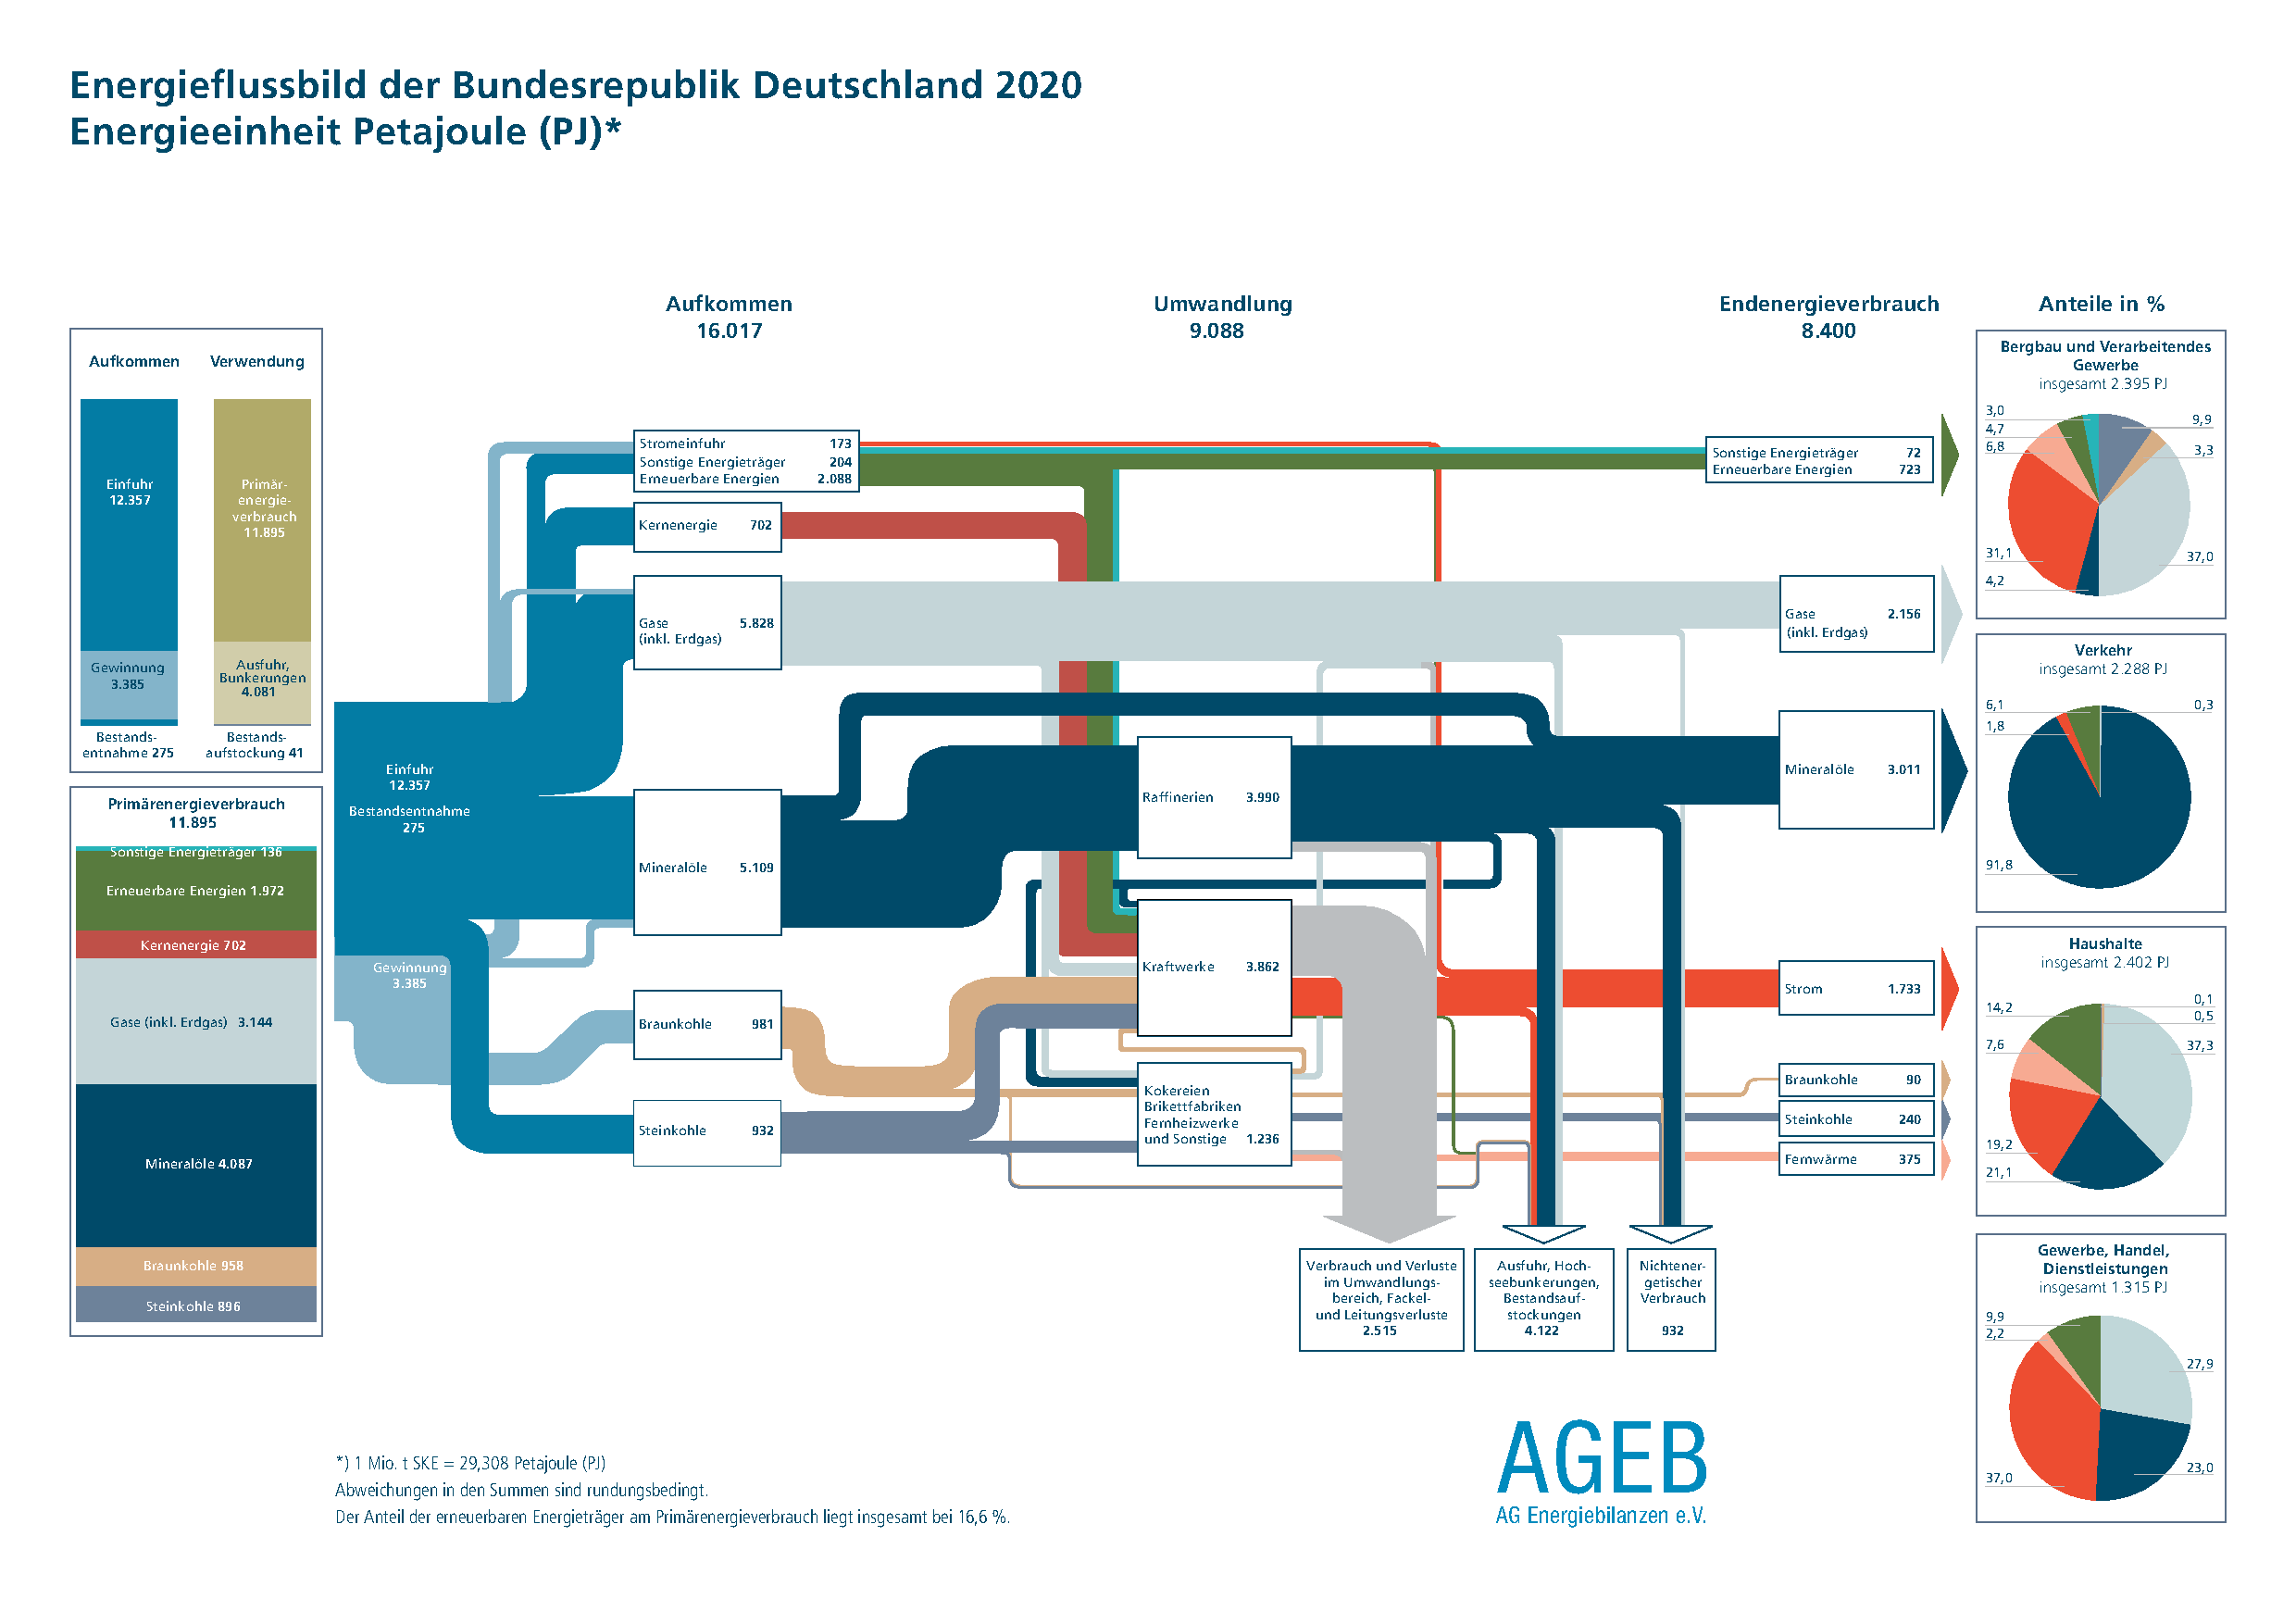
\includegraphics[width=0.9\textwidth]{../pres/fig/Energieflussbild-2020_PJ_lang_DE_20220401.pdf}
\caption{Energiefluss für Deutschland 2020 \cite{energieflussbild}}
\label{fig:energiefluss}
\end{figure}

Deutschland hat insgesamt einen Gasbedarf von 905 TWh pro Jahr \cite{clausen2022}. Dies entspricht 27\% der Gesamtprimärenergienachfrage und macht Gas damit zum zweitwichtigsten Primärenergieträger nach Mineralöl. Gas wird zum größten Teil (66\%) zur Wärmeproduktion eingesetzt. 

Wie in \autoref{fig:energiefluss} erkennbar, wird Gas außerdem mit einem signifanten Teil in Kraftwerken zur Stromproduktion verwendet, zu geringem Teil ausgespeichert und zu großen Teilen im verarbeitenden Gewerbe eingesetzt. 

Die nächsten Abschnitte adressieren die Speicherung von Erdgas, sowie welche Alternativen zum Erdgasverbrauch es für die genannten Anwendungsbereiche gibt und in welchem Zeithorizont diese umsetzbar sind.

\subsubsection{Gasspeicher}

Deutschland verfügt mit 265 TWh über die höchste Gasspeicherkapazität der EU \cite{iwd}. Den Großteil dieser Kapazität machen 51 unterirdische Kavernenspeicher aus. Deren Zweck ist es, Lieferengpässe beim Erdgas auszugleichen. Da die Kapazität etwa 30\% des Jahrverbrauchs ausmacht, sind sie dafür auch durchaus geeignet.
Es wird darauf abgezielt die Speicher zu Beginn des Winters so voll wie möglich zu haben. Im Normalfall ist die Füllquote auch bei 95\%. Im Winter 2021 waren die Speicher allerdings nur zu 66\% gefüllt. Ein Viertel der deutschen Gasspeicher gehörten dem russischen Staatskonzern Gazprom. Diese Speicher wurden über das letzte Jahr kaum befüllt. So waren schließlich auch 05.~März 2022 zu Beginn des russischen Angriffskrieges auf die Ukraine dazu, dass die Speicher nur noch zu 27\% gefüllt waren. Im Normalfall sind sie im selben Zeitraum 50-80\% gefüllt.

Die deutschen Erdgasspeicher stehen allesamt bisher in privatem Besitz \cite{leo}. Aus rein ökonomischer Sicht ist es unter Umständen aber zu riskant die Gasspeicher zu befüllen. Wenn zum Beispiel Gazprom bei vollem Speicherstand in Zeiten hoher Nachfrage den Gasmarkt mit billigem Gas flutet, erleiden die Gasimporteure und Speicherbetreiber einen hohen wirtschaftlichen Schaden, da sie das gespeicherte Gas nicht verkaufen können. Auf der anderen Seite sind ungefüllte Speicher wie in diesem Jahr erkenntlich elementar für die Stabilität und Unabhängigkeit der deutschen Energieversorgung. Deswegen sollte die Handhabe der deutschen Speicher so reguliert werden, dass sich eine Einspeicherung im Sommer stets lohnt oder gezwungenermaßen vonstatten geht.

\subsubsection{Wärmeversorgung}

Die größte Rolle spielt Gas bei der Wärmeversorgung. 
Es wird zwischen der Raumwäreversorgung (28\%), der Prozesswärme in der Industrie (26\%) und der Wärmeversorgung im Dienstleistungssektor (12\%) unterschieden. Tatsächlich sind 49,5\% der deutschen Heizungen noch Gasheizungen.  

Im Wärmesektor herrscht ein beschränktes aber nicht zu vernachlässigendes Potential für kurzfristige Energieeinsparungen. Eine Reduktion Temperatur aller mit Erdgas beheizten Wohnungen der EU um 1 Grad Celsius entspricht einer Einsparung im Erdgasverbrauch um 100 TWh pro Jahr \cite{iea2022}.

Die sowieso schon hohen Gaspreise sorgen sowohl in den Haushalten wie auch in der Wirtschaft durch Verhaltensänderung bereits für Einsparungen \cite{tagesschau-gasverbrauch}. Zwischen Januar und Mai 2022 ist der Gasverbrauch 14\% niedriger als im Jahr 2021. Dafür sind auch die milderen Temperaturen im Frühjahr verantwortlich. Wenn man diese in die Berechnung miteinbezieht sank der Verbrauch immernoch um 6,4\%. Haushalte wie Unternehmen denken stärker darüber nach ob und welche Fläche beheizt werden muss.

Deswegen sollten die Preis-Anreize auch beibehalten werden. Kontraproduktiv wäre es, in dieser Situation z.B. die Mehrwertsteuer auf fossile Energie zu reduzieren, da dies die Anreize außer Kraft setzen würde. Um sozialen Verwerfungen entgegenzuwirken kann stattdessen auf ein pauschales oder sozial gestaffeltes Energiegeld gesetzt werden \cite{clausen2022}. Diese Idee wird auch häufig im Rahmen des CO2-Bepreisung eingebracht. Die Einnahmen aus dem CO2-Preis können für die sozialverträgliche Kompensation der Mehrbelastung genutzt werden, indem jeder Bürger ein monatliches oder jährliches Energiegeld erhält. Wer wenig Energie verbraucht (was für die meisten Geringverdiener zutrifft) erzielt dabei in der Gesamtrechnung einen Gewinn. Für alle bleibt der Anreiz zum Energiesparen erhalten \cite{leo}. Je stärker und länger die Energiepreise wachsen, desto wichtiger wird eine solche finanzielle Kompensation.

Eine technologische Form der Wärmeeinsparung ist das intelligente Heizen: über vernetzte Thermostatventile und Heizungsteuerungen kann durch informierte Entscheidungen darüber welche Räume wann zu heizen sind bis zu 20\% der Heizenergie gespart werden \cite{clausen2022}. Diese Technologie ist außerdem breit verfügbar und mit geringen Investitionen verbunden. Sie sollte deswegen stärker incentiviert werden, zum Beispiel durch Subventionen oder Pflichten.

Die Effizienz von (Gas-)Heizungen ist über die letzten Jahr gestiegen. Die daraus resultierende Energieeinsparung wurde jedoch durch den signifikanten Anstieg in der Wohnfläche pro Person kompensiert. Wohnte eine durchschnittliche Person in Deutschland 1991 noch auf 34,9 Quadratmetern, wohnt sie 2020 nun auf 47,4 Quadratmetern \cite{clausen2022}. Erhöhte Energiepreise könnten langfristig dafür sorgen, dass sich dieser Trend wieder etwas umkehrt.

Eine weitere längerfristige Maßnahme zur Heizenergieeinsparung ist die Sanierung von Altbauten. 
Dazu zählt die Isolation von Gebäuden, aber auch die effizientere Wärmeverteilgung durch moderne Pumpen \cite{ei1}.
Momentan werden jährlich nur 1\% der EU-Gebäude saniert \cite{iea2022}. Steigende Preise dürften diese Maßnahmen incentivieren, doch es muss auch dafür gesorgt werden, dass Lieferketten und Fachkräfte für standardisierte Upgrade sichergestellt sind. Es kann auch darüber nachgedacht werden, staatliche Fördermaßnahmen einzurichten, um diese Anpassungen noch stärker zu motivieren.

Eine grundlegend anderer Ansatz zur Einsparung von Erdgas in der Warmeversorgung ist der Ersatz der Gasheizung. Auch diese Maßnahme ist kurzfristig schwer umzusetzen, insbesondere in der Prozesswärmeversorgund der Industrie \cite{leo}. Grundlegend gibt es folgende Alternativen: der Anschluss an Wärmenetze, der Ersatz durch regenerative Wärmequellen, die Elektrifizierung über Wärmepumpen oder der Einsatz von (grünem) Wasserstoff in dezentralen Gasheizungen \cite{clausen2022}.
Von diesen Optionen ist nur die letzte aufgrund hoher Effizienznachteile im Vornherein auszuschließen. Beim Einsatz von 100 kWh erneuerbarem Strom kann durch die Umwandlung in Wasserstoff mit anschließender Verbrennung 
nur 61 kWh Wärme produziert werden. Eine Wärmepumpe produziert im Vergleich 135 - 270 kWh, je nach Außentemperatur \cite{agora-wasserstoff}.

Konventionelle Kraftwerke produzieren Strom durch die Verbrennung (fossiler) Energieträger. Sie heizen damit Wasser zu Dampf der eine Turbine antreibt, die über einen Generator Strom produziert. Dabei bleibt ein signifikanter Teil der Energie in Form von Abwärme ungenutzt. Wird statt der seperaten Produktion von Wärme, diese Abwärme lokal genutzt oder über Wärmenetze verteilt spricht man vom Prinzip der Kraft-Wärme-Kopplung \cite{kwk}. Dieses ist in \autoref{fig:kraft-waerme-kopplung} dargestellt. 
Um den Gasverbrauch zu reduzieren, sollte also das Potenzial Wärmenetze auszubauen oder zusätzliche Gebäude an diese Netze anzuschließen ergründet werden.
Zum Ausbau der Wärmenetze zählt auch der Aufbau von Quartierswärmespeichern, wie Erdbeckenwärmespeicher, die die lokale Wärmeversorgung vor allem bei volatiler regenerativer Energieversorgung stabilisieren können \cite{clausen2022}.

\begin{figure}
\centering
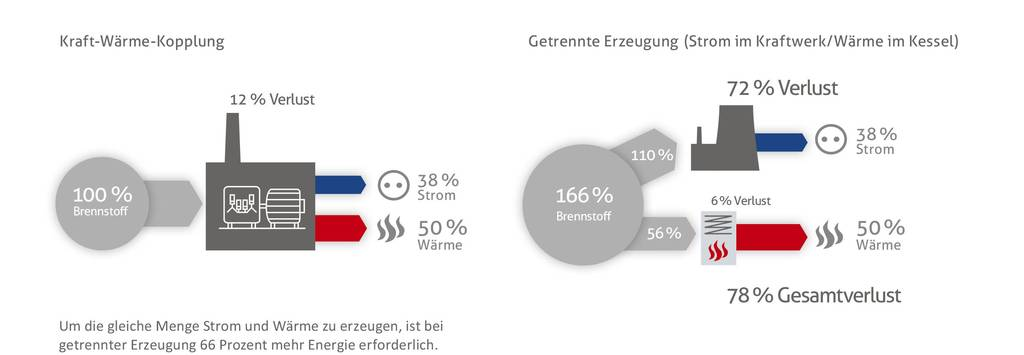
\includegraphics[width=12cm]{../pres/fig/kraft-waerme-kopplung.jpg}
\caption{Potenzial der Kraft-Wärme-Kopplung \cite{kwk}}
\label{fig:kraft-waerme-kopplung}
\end{figure}

Wärmenetze können nämlich auch durch regenerative Wärmequellen gespeist werden.
Dazu zählen vor allem die Solarthermie und die Geothermie. Die Solarthermie hat eine hohe Flächeneffizienz und die niedrigsten Treibhausgas-Vermeidungskosten, ist kombinierbar mit landwirtschaftlicher Nutzung (Agri-Solarthermie) und hat kann für etwa 60 TWh/a der Niedertemperaturprozesswärme eingesetzt werden \cite{clausen2022}. 

Bei der Geothermie wird die in der Erdkruste gespeicherte Wärme durch Wärmetauscher übertragen. Dazu sind Bohrungen in unterschiedlichen Tiefen möglich oder sinnvoll. Dies hängt auch stark von der lokalen Präsenz von Wärmeanomalien ab. So ist Deutschland ungeeignet für den Einsatz von Hochenthalpie-Anlagen, die hohe Temperaturen in vergleichsweise geringer Tiefe abgreifen können und für die Wärme oder gar Stromproduktion nutzen. Deswegen ist die in Deutschland insgesamte installierte Leistung (27 MW 2015) durch Geothermieanlagen im internationalen Vergleich mit Ländern wie den Philippinen (1870 MW) oder Island (665 MW) deutlich geringer \cite{ei1}. Doch für die Wärmeversorgung eignen sich auch Niederenthalpie-Anlagen, die keine besonderen Wärmeanomalien aber häufig tiefe Bohrungen voraussetzen. Solche Anlagen bei 400m Tiefe haben in Deutschland ein Potential von 100-300 TWh/a für die Wärmeproduktion \cite{clausen2022}.
Der Vorteil der Geothermie ist deren Unabhängigkeit von Eingabeenergie und Stabilität. Schwierigkeiten sind die hohe Kosten bei tiefen Bohrungen, salziges korrosives Wasser (Ausnahme: Süddeutschland) und Risiken seismischer Aktivität bei der Tiefengeothermie \cite{ei1}.

Eine weitere regenerative Wärmequelle ist die Biomasse. Die Verbrennung von Holz ist die geschichtlich am weitesten zurückreichende Methode des Heizens und auch heute noch mit 68\% 2017 den größten Teil in der erneuerbaren Wärmeversorgung aus \cite{ei1}. Die flächendeckende Anwendung von Biomasse für die Wärmeversorgung ist im dicht besiedelten heutigen Deutschland mit immer schwächer nachwachsenden Wäldern infrage zu stellen. Prinzipiell ist das Anpflanzen und Verbrennen von Bäumen zwar klimaneutral, da die Bäume beim Wachsen CO2 binden, das beim Verbrennen freigesetzt wird. Bei der Produktion und dem Transport fallen jedoch Treibhausgase an, die die in Summe zu einem Plus an Treibhausgasemissionen führen.
Dies gilt insbeondere für das Heizen mit Pellets, die häufig über lange Wege transportiert werden.
Erneuerbar ist das Heizen mit Holz natürlich auch nur dann wenn auch nur no so viele Bäume entnommen werden wie nachwachsen, was in Zeiten des Klimawandels und Waldsterbens bei hoher Nachfrage sehr unrealistisch ist.
Neben Holz hat Biogas in Deutschland mit 10\% 2017 den zweitgrößten Anteil an der erneuerbaren Wärmeversorgung. Der Anbau von Energiepflanzen zur Produktion von Biogas steht über den Flächenverbrauch jedoch im Konflikt mit der Nahrungsmittelversorgung und kann deswegen jedenfalls nicht weiter erhöht werden.

\begin{figure}
\centering
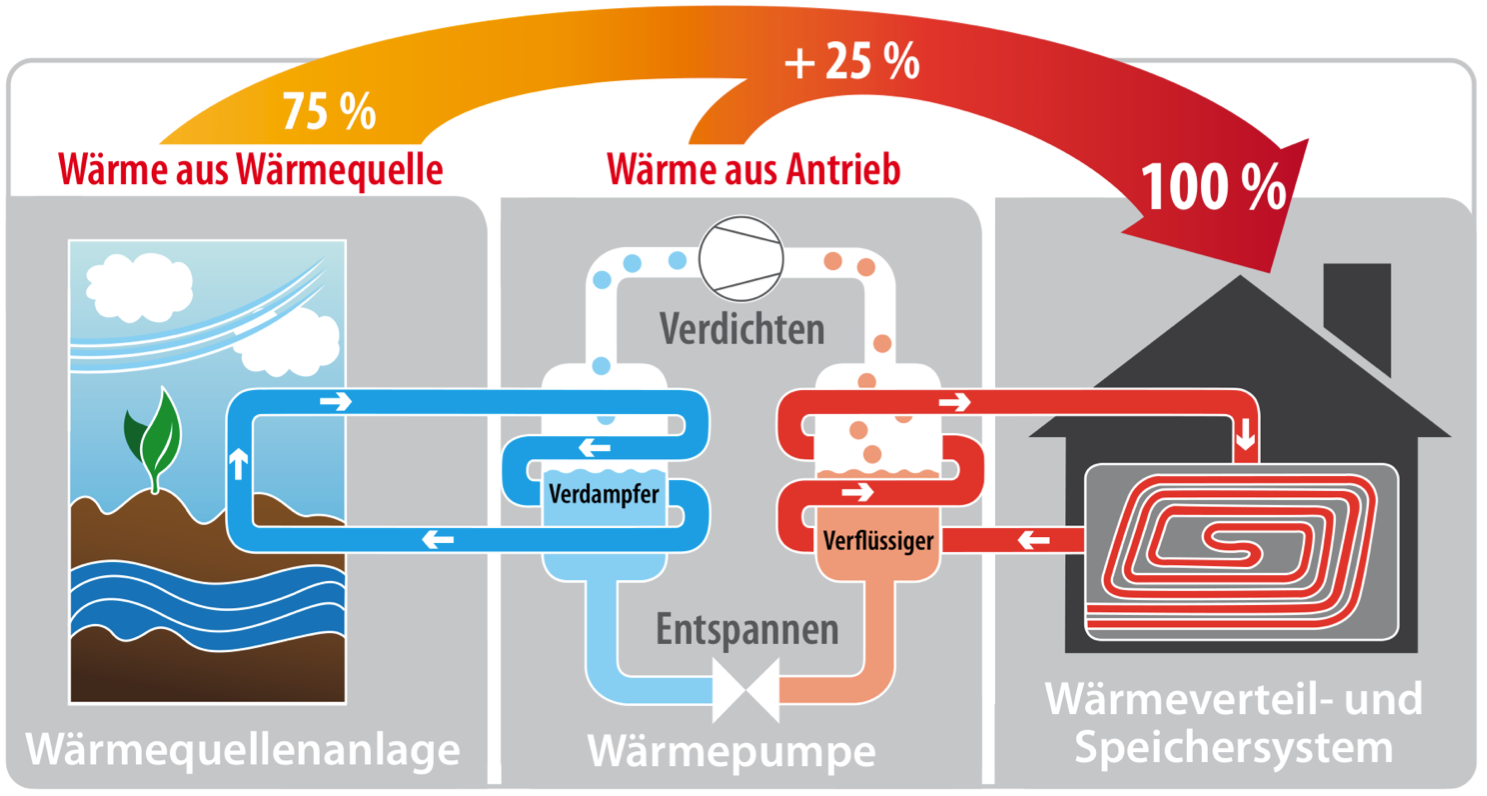
\includegraphics[width=12cm]{../pres/fig/waermepumpe.png}
\caption{Funktionsprinzip der Wärmepumpe \cite{ei1}}
\label{fig:waermepumpe}
\end{figure}

Gebäude können auch rein elektrisch geheizt werden. Neben ineffizienten Brennstäben bietet kann dafür eine Wärmepumpe verwendet werden. Dessen Funktionsprinzip ist in \autoref{fig:waermepumpe} dargestellt. Eine Wärmepumpe funktioniert nach dem umgekehrten Prinzip eines Kühlschranks. Sie verwendet elektrische Leistung um thermische Energie aus einem Kältereservoir in eine Wärmereservoir zu übertragen. Dabei versteht man das Kältereservoir auch als Wärmequelle, weil die darin enthaltene thermische Energie mit verwendet wird. Die ausgegebene thermische Energie ist dadurch im Betrag höher als die eingegebene elektrische Energie. Deswegen wird die Effizienz einer Wärmepumpe nicht in Form eines Wirkungsgrades $\in [0,1]$ sondern in Form einer Leistungszahl $\epsilon > 1$ angegeben \cite{ei1}. Sie eignet sich als Ersatz für fossile Heizungen in der Wärmewende, weil sie direkt die durch Photovoltaik oder Windkraft gewonnene elektrische Energie verwenden kann. Langfristig sollen mit Wärmepumpen 60-70\% des Wärmebedarfs gedeckt werden können. Sie können bis 2030 25-75\% des russischen Erdgases einsparen \cite{clausen2022}. Im Neubau war 2020 die Wärmepumpe zum ersten mal die meistverbauteste Heiztechnologie \cite{statista-neubau-heizung}. Im Bestand machen sie aber noch immer nur weniger als 3\% der verbauten Heizungen aus. Die Gasheizung ist mit etwa 50\% seit 1995 die meistverbauteste Heizung \cite{statista-bestand-heizung}. Womöglich auch deswegen waren auch 2021 nur 18\% der ausgetauschten Heizsysteme Wärmepumpen \cite{clausen2022}. 
Die Wärmewende und die Unabhängigkeit von russischem Erdgas erfordern eine massive Beschleunigung im Einbau von Wärmepumpen. Dafür sind qualifizierte Fachkräfte notwendig. Die Regierung sollte eine Ausbildungsoffensive im Handwerk für Wärmepumpeninstallateure und Elektrofachkräfte aufbauen, die auch in der Lage sind, die Wärmepumpen stromseitig an eine PV-Anlage anzuschließen. 
Die Elektrifizierung der Mobilität mit Elektrofahrzeugen und die Elektrifizierung der Wärmeproduktion über Wärmepumpen erfordern darüber hinaus einen Ausbau der erneuerbaren Stromproduktion um das Ziel bis 2030 zu halten 80\% des Stroms aus erneuerbaren Quellen zu decken \cite{clausen2022}. Bis 2050 muss dafür die Stromproduktion aus Sonne und Wind zum Jahr 2020 verdreifacht werden \cite{agora-wasserstoff}.
Die Förderung von Erdgas-Brennwertheizungen sollte vollständig beendet werden. Momentan kann man für den Wechsel auf eine Gasheizung noch 20-40\% Förderung vom Staat erhalten -- wenn diese entwerder als ``renewable ready'' Heizung innerhalb von 2 Jahren um eine erneuerbare Quelle ergänzt wird oder sofort als Gas-Hybridheizung mit einer erneuerbaren Quelle wie Solarthermie kobminiert wird \cite{gasheizung-foerderung}. Die Idee hinter einem Einbau dieser Systeme ist verständlich. Wärme wird bevorzugt aus der Solarthermie bezogen, für die kalten und dunklen Wintermonate kann man sich aber auf das sicher verfügbare Gas verlassen. Langfristig kann das keine nachhaltige Alternative sein, was das Gas nur sehr teuer durch energieintensiven Wasserstoff ersetzt werden kann \cite{agora-wasserstoff}. Ab einem gewissen Zeitpunkt könnten die Gasheizungen aufgrund der Klimaneutralität tatsächlich auch die Betriebsgenehmigung verlieren, sogar über ein Verbot vom Einbau von Öl- und Gasheizungen nachgedacht werden kann. Der aktuelle Koalitionsvertrag sieht bereits vor, dass ab 2025 nur noch Heizungen eingebaut werden dürfen, die auf 65\% Erneuerbaren betrieben werden \cite{clausen2022}.

Ein allgemeines Problem bei vielen dieser Maßnahmen ist das Vermieter-Mieter-Dilemma \cite{agora-mieterschutz-klimaschutz}. 
Der Mieter bezahlt monatlich den Preis für die zur Heizung von Raum und Wasser notwendigen Energie.
Doch der Vermieter entscheidet über energetische Sanierungen oder den Ersatz der Heizung durch effizientere oder nachhaltigere Alternativen. Diese Investitionen können sich für den Vermieter aber zum Teil gar nicht refinanzieren, da dieser von der Investition nicht genug Geld zurück erhält. Es dürfen 11\% der Investitionssumme über die Kaltmiete auf den Mieter umgelegt werden. Auch für den Mieter ist die Investition dann aber nicht unbedingt immer finanziell erstrebenswert, wenn nämlich die Sanierung nicht genug Energie einspart um die Mehrkosten der Miete zu decken. Für den Vermieter ist auch nur entscheidend wie teuer, nicht wie effektiv die Sanierung war. Ein alternatives Modell ist die Warmmiete mit Temperaturfeedback. Ist im Mietvertrag geregelt, dass sich der Vermieter, um die Wärmeversorgung kümmert und eine Mindesttemperatur bereitstellt, kann dieser Geld einsparen indem er Investitionen zielt. Dieses Konzept ist in Schweden üblich. Dort sind auch seit 2000 die Emissionen der Haushalte um 95\% gesunken.

\subsubsection{Stromproduktion}
\label{sec:Stromproduktion}

Zur Stromproduktion wurden 2021 171 TWh (19\%) vom Erdgas in Gaskraftwerken in 95 TWh Elektrizität umgewandelt \cite{clausen2022}. Wendet man darauf den Anteil der russischen Erdgasimporte (55\%) an, sind so schnell wie möglich 52 TWh/a Strom anderweitig zu produzieren.

Es gibt zwei Arten von Gaskraftwerken. Das einfach Gaskraftwerke wandelt Gas mittels Gasturbine unter sehr hohen Temperaturen in Strom um. Auch die Abwärme ist bei diesen Kraftwerken sehr hoch. Die sogenannten Gas- und Dampkraftwerke nutzen diese Abwärme nach dem Prinzip der Kraft-Wärme-Kopplung in einem zweiten Dampf-basierten Energiewandelprozess um zusätzlichen Strom zu produzieren. Dadurch ist das Gas- und Dampfkraftwerk unter allen Kraftwerkstypen mit einem Wirkungsgrad von 60\% die effizienteste Art \cite{ei1}. Dieses Attribut ist natürlich nur für fossile Kraftwerke und Kernkraftwerke wirklich relevant, da erneuerbare Kraftwerke mit Ausnahme der Biomassebasierten Kraftwerke kostenlose und unlimitierte Eingabeenergie verwenden.
Das spiegelt sich auch darin wieder, dass Gaskraftwerken gegenüber anderen auf fossiler Energie basierenden Kraftwerken weniger Treibhausgasemissionen und Luftschadstoffe verursachen \cite{uba-co2}. Das stammt jedoch auch daher das die Verbrennung von Methan im Allgemeinen weniger Treibhausgasemissionen verursacht als die Verbrennung von Kohle oder Öl.

Das bedeutet in Summe, dass wenn Strom aus Gaskraftwerken durch Strom aus Kohlekraftwerken ersetzt wird, zum einen durch Niedereffizienz mehr Primärenergie benötigt wird und die Treibhausgasemissionen in der Stromproduktion höher sind. Kohle und Öl stehen jedoch im Kontrast zu Alternativen für einen Ersatz auch zur Verfügung \cite{iea2022}. Die Verbrennung deutscher Kohle statt russischem Gas würde 27 Mt CO2 mehr verursachen als die Verbrennung von Gas \cite{leo}. 
Die Emissionen der europäischen Stromproduktion sind aber durch den Emissionshandel (ETS) fest nach oben limitiert. Das bedeutet, dass die Kohleverstromung die Preise erhöht, aber in Summe nicht die Emissionen, da diese anderweitig eingespart werden müssen. Diese Situation stellt natürlich den geplanten Kohleausstieg 2038 infrage. Es bleibt aber weiterhin sinnvoll an diesem festzuhalten, unter anderem deswegen, weil über die Jahre 2017 bis 2021 40 bis 50\% der Steinkohle aus Russland importiert wurde \cite{steinkohle-import}.

Eine weitere Option für Deutschland liegt in der Verzögerung des geplanten Laufzeitendes am 31.~Dezember 2022 der letzten drei verbleibenden Atommeiler. Diese produzieren im Jahr 2022 eine geplante Elektrizitätsmenge von etwa 30 TWh \cite{kernkraftwerke-rest}. Könnten diese im selben Modus weiterbetrieben werden, würden sie damit mehr als die Hälfte des Ausfall oder Vermeidung russischen Erdgases verbleibenden Strombedarfs decken. Die Verlängerung ihrer Laufzeiten gestaltet sich infolge der schon vorbereiten Abschaltung als technisch herausfordernd und ökonomisch sehr aufwendig \cite{leo}. Dazu kommt, dass die EU auch beim Uran stark von Russland abhängig ist \cite{spigel-uran}. 40\% des in der EU genutzten Urans wird aus Russland und Kasachstan importiert. Gravierend ist, dass Russland 26\% des \textit{angereicherten} Urans herstellt und für Betreiber von WWER-Rekatoren der einzige Lieferant von sechseckigen Brennstäben ist.
Würde Deutschland die Laufzeit der Atomkraftwerke verlängern wäre zu klären, woher das Uran importiert werden soll, wenn gerade EU-weit versucht wird auf andere Lieferländer auszuweichen.

Was bleibt ist die Substitution durch Kraftwerke aus erneuerbaren Energien. Hierbei sind in Deutschland vor allem die Photovoltaik und die Windkraft relevant. Nach Berechnungen ersetzt 1 GW installierter Windkraftleistung 5,6 TWh/a Gas (bei 2800 Volllaststunden) und 1 GW Leistung aus Photovoltaik ersetzt 1,8 TWh/a Gas (bei 920 Volllaststunden) \cite{clausen2022}. Der Ersatz der 45 TWh Strom aus russichem Erdgas erfordert also einen Zubau von 30-40\% der bisher installierten Kapazität an PV und Windenergie. Das verdeutlicht, dass diese Alternative leider nur mittel- bis langfristig realistisch ist. Eine mögliche Maßnahmen ist jedoch, die 5 GW (= 28 TWh/a) Windkraft, die momentan im Genehmigungsstau stehen als Notfallmaßnahme beschleunigt zuzulassen \cite{clausen2022}. Allgemein sollte versucht werden starre Regularien und langsame Genehmigungsverfahren zu vereinfachen und zu beschleunigen. Dabei kann es helfen administrative Kapazität aufzubauen, klare Deadlines festzulegen und die Prozesse zu digitalisieren \cite{iea2022}. Zusätzlich kann die Installation gefördert werden oder bei der Photovoltaik auf Neubauten sogar verpflichtet werden.

\begin{figure}
\centering
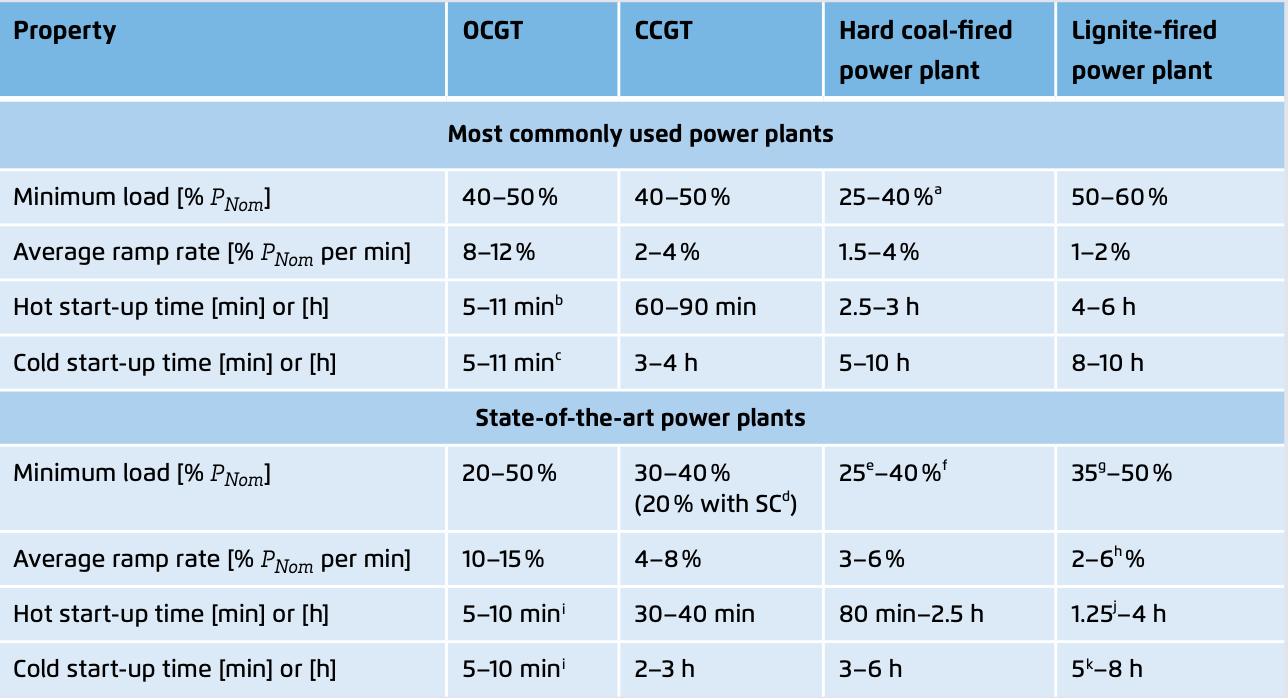
\includegraphics[width=12cm]{../pres/fig/flexibility_power_plants.png}
\caption{Flexibilität unterschiedlicher Kraftwerkstechnologien nach Beschleunigungsrate und Kalt- und Warmstartzeit \cite{agora}}
\label{fig:flexibility}
\end{figure}

Ein weiterer Aspekt von Gaskraftwerken ist, dass sie im Vergleich zu Kohle- und Kernkraftwerken sehr flexibel betrieben werden können. Die dafür wichtigen Parameter sind wie schnell die produzierte Leistung erhöht werden kann (Ramp rate) und wie lange ein Kraftwerk für einen Kalt- oder Warmstart benötigt (Hot- oder Cold-start-up time). Wie in \autoref{fig:flexibility} erkennbar, benötigen Gaskraftwerke für beides nur etwa 5-10 Minuten und sind damit deutlich schneller als Gas- und Dampkraftwerke welche wiederum etwas schneller als Kohle- und Kernkraftwerke sind. Im Stromnetz ist die Frequenzstabilität ein wichtiger Faktor. Gaskraftwerke eignen sich gut dafür Spitzenlast durch kurzfristig erhöhte Produktion zu decken und helfen damit das Stromnetz gegen Ausfälle zu sichern \cite{ei1}.
Gaskraftwerke werden deshalb im Stromsektor als Haupt-Flexiblitätsquelle vor allem im Wandel zu mehr volatiler Stromproduktion durch Wind und Sonne betrachtet \cite{iea2022}. Daher rührt auch die Bezeichnung von Gas als Übergangstechnologie.

Soll (russisches) Erdgas ersetzt werden muss also nicht nur die produzierte Strommenge, sondern auch die durch sie bereitgestellte Regelleistung ersetzt werden. Das demonstriert über die bereits beschriebenen Probleme hinaus, warum Kernkraftwerke den Strom aus Gaskraftwerken nicht äquivalent ersetzen können.
Doch dieses Problem haben auch Kohlekraftwerke, vor allem jedoch betrifft es die Erneuerbaren. Ein Zubau von Erneuerbaren erhöht sogar die erforderliche Regelleistung im Netz um ihre Volatilität auszugleichen. Deswegen müssen andere (und neue) Möglichkeiten der Frequenzstabilisierung auf die Wege gebracht werden. 
Eine Option ist lastseitig auf einen erhöhten Verbrauch zu antworten. Bestimmte Stromverbraucher eignen sich dazu in ihrer Last unterbrochen zu werden. Die Industrie kann Netzbetreibern eine solche Unterbrechbarkeit als Dienstleistung anbieten \cite{ei1}. Die bereits genannte fortschreitende Elektrifizierung von Elektrofahrzeugen und Wärmepumpen eignet sich gut für solche Lastunterbrechungen, da Autos häufig lange Standzeiten haben und Räume und Wassertanks die Wärme speichern. Eine weitere mögliche und sowieso nötige Investition ist der Aufbau von kurz- und langfristigen Stromspeichern. Als kurzfristige Stromspeicher eignen sich Batterien. Diese sind ähnlich zu Gaskraftwerke gut steuerbar und können diese Flexibilität im Netz gut ersetzen \cite{clausen2022}. Um die Dunkelflaute mit wenig Wind und Sonne, die bis zu Wochen dauern kann zu überbrucken wird es langfristig auch Langzeitspeicher brauchen. Die dafür geeignetste Technologie ist die Umwandlung in Wasserstoff, Speicherung in den genannten großen Kavernenspeichern und Rückverstromung in Gaskraftwerken oder Brennstoffzellen \cite{leo}. Doch Wasserstoff ist nicht nur als Energiespeicher gefragt.

\subsubsection{Erdgas in der Chemieindustrie}

Die Chemieindustrie machte 2021 15,4\% des Erdgasbedarfs in Deutschland aus \cite{vci2022}. Erdgas ist der wichtigste Energieträger in der Industrie. 99,3 TWh (73\%) wurden 2021 energetisch und 36,8 TWh (27\%) stofflich eingesetzt. Bei der Produktion chemischer Produkte benötigen bestimmte Reaktionen eine energetische Eingabe in Form von Wärme oder Strom. Beim stofflichen Einsatz wird das Methan benötigt, aus dem Erdgas zum großen Teil besteht. Das prominenteste Beispiel dafür ist die Ammoniakherstellung. Ammoniak wird weltweit zu 99\% nach dem Haber-Bosch Verfahren produziert \cite{smil}. Dabei wird Methan mittels Dampfreformierung unter Zufuhr von Wasser und Energie in Wasserstoff umgewandelt. Der Ammoniak entsteht dann durch eine Reaktion von Wasserstoff mit Stickstoff aus der Luft unter Wärmezufuhr. Ammoniak ist ein wichtiger Rohstoff für die mineralische Düngemittelproduktion und damit für die Agrarwirtschaft. Es könnte versucht werden die mineralischen Düngemittel durch organische Düngemittel zu ersetzen. Es is jedoch fraglich, ob die Nachfrage nach Lebensmittel der wachsenden globalen Bevölkerung mit diesen gestillt werden kann.

Die für die Chemieindustrie nötige Energie in Form von Wärme und Strom kann man analog zu den vorherigen Abschnitten zu ersetzen versuchen. Durch diese Industrie erhöht sich dementsprechend anteilig nochmal die zu ersetzende Menge an Erdgas. Doch wenn hier Methan als chemischer Stoff eingesetzt wird, stellt sich die Frage wie dieser überhaupt ersetzt werden kann.

Wasserstoff kann neben der Dampfreformierung auch durch Elektrolyse produziert werden. Dabei wird Wasser unter Zufuhr von Strom in Wasserstoff und Sauerstoff umgewandelt. Stammt der zugeführte Strom aus erneuerbaren Energien ist von grünem Wasserstoff die Rede. Die Elektrolyse wäre wie gesagt auch der Weg temporär überschüssigen erneuerbaren Strom für längere Zeiten zwischenzuspeichern. Bis 2030 wird so gewonnener Wasserstoff aber nur in sehr geringen Maßen verfügbar sein \cite{kopernikus}. Um die Nachfrage nach Wasserstoff zu decken wird ein zusätzlich zur Elektrifizierung nochmal stärkerer Zubau an Erneuerbaren Energien notwendig sein \cite{agora-wasserstoff}. Insgesamt ist also erforderlich, dass die installierte Leistung an Wind- und Solarstrom bis 2040 vervierfacht wird. 
Zusätzlich müssen Elektrolyseure installiert werden, bevorzugt in der Nähe großer (Offshore-)Windparks \cite{ei1}. Für einen Transport des produzierten Wasserstoffs eignet sich das existierende Gasnetz, wenn der Wasserstoff vor der Einspeisung methanisiert wird.

Auch ein Import von Wasserstoff aus Regionen mit höherer Verfügbarkeit an erneuerbarem Strom ist denkbar. Deswegen ist es wichtig, dass die momentan gebaute Infrastruktur zum Import von Flüssiggas sich auch zum Import von Wasserstoff eignen wird \cite{leo}.
Der Preis für Wasserstoff liegt derzeit mit 100 Euro pro MWh deutlich über dem 40 Euro pro MWh für Erdgas \cite{rnd}. Doch auch in Zukunft wird der Energieträger teuer bleiben.

Aus diesem Grund ist vom Gebrauch von Wasserstoff abzusehen, wo er nicht drigend benötigt wird. Wie besprochen gibt es in der Wärmeversorgung von Haushalten mit der Wärmepumpe eine effizientere Alternative den Strom aus Erneuerbaren direkt zu nutzen. In der Ammoniak- und Stahlproduktion hingegen gibt es bisher keine Alternativen zum Wasserstoff \cite{kopernikus}.

\subsection{Fazit}

Die Analyse der alternativen Importländer zeigt, dass die großen Mengen an aus Russland importierten Gas schwer schnell zu ersetzen sind. Durch weiterhin entschiedenes und schnelles Handeln könnte es aber möglich sein, auch einen Lieferstopp vonseiten Russlands auszuhalten, wenn genug Flüssiggas beschafft und transportiert werden kann, die Gasspeicher über den Sommer gefüllt werden, Erdgas im Stromsektor durch Kohle ersetzt wird und die Mehrbelastungen bei Bürgern durch höhere Preise mit einem Energiegeld abgefedert wird. 

Längerfristig geht die Liberalisierung von russischem Erdgas Hand in Hand mit der Transformation zur Klimaneutralität. Um den Verbrauch der Sektoren Wärme, Strom und Chemieindustrie zu adressieren müssen die erneuerbaren Energien massiv ausgebaut, die Wärmeproduktion elektrifiziert, Verbraucher flexibilisiert, Batteriespeichern installiert, Elektrolyseuren aufgebaut und das Gasnetzes zum Transport von Wasserstoff ertüchtigt werden.